
\chapter{ಗ್ರೇಟ್​ ಟ್ರಿಗನಮಿಟ್ರಿಕಲ್​ ಸ್ಟೇಷನ್​ಗೆ ಬೇಕು ಎತ್ತರದ ಬಂಡೆ, ಬೆಟ್ಟ ಅಥವಾ ಗೋಪುರ}

ಗ್ರೇಟ್​ ಟ್ರಿಗನಮಿಟ್ರಿಕಲ್​ ಸರ್ವೇ ಸ್ಟೇಷನ್​ಗಳ ಆಯ್ಕೆಯನ್ನು ಹೇಗೆ ಮಾಡಬೇಕೆಂಬುದಕ್ಕೆ ಮಾರ್ಗದರ್ಶಿ ಸೂತ್ರಗಳಿವೆ. ತ್ರಿಭುಜದ ಬಿಂದುಗಳು ಪರಸ್ಪರ ಗೋಚರಿಸಬೇಕು. ಸುಲಭವಾಗಿ ತಲುಪುವಂತಿರಬೇಕು. ಅಡ್ಡ ಬರುವ ನೆಲ ಅಗೆತ, ಮರ ಕಡಿತ, ಗೋಪುರ ನಿರ್ಮಾಣ ಈ ಕಾರ್ಯಗಳು ಸಾಧ್ಯವಾದಷ್ಟೂ ಕನಿಷ್ಠವಾಗಿರಬೇಕು. ಸಮಬಾಹು ತ್ರಿಭುಜಗಳಿಗೆ ಸಮೀಪವಾದ ತ್ರಿಭುಜಗಳಾಗುವಂತೆ ಸ್ಟೇಷನ್​ಗಳಿರಬೇಕು. ಸ್ಟೇಷನ್​ಗಳು ಈ ರೀತಿ ಇದ್ದಾಗ, ಓದಿದ ಕೋನಗಳಲ್ಲಿ ಏನಾದರೂ ಅಲ್ಪಾತಿ ಅಲ್ಪ ದೋಷವಿದ್ದರೂ, ಈ ಕೋನಗಳನ್ನಾಧರಿಸಿ ಮಾಡುವ ಬಾಹುಗಳ ಲೆಕ್ಕಾಚಾರದಲ್ಲಿ ದೋಷ ಕಡಿಮೆ ಇರುತ್ತದೆ. ಯಾವುದೇ ಕೋನವು \enginline{30°} ಗಿಂತ ಚಿಕ್ಕದು ಅಥವಾ \enginline{90°} ಗಿಂತ ದೊಡ್ಡದು ಇರಬಾರದೆನ್ನುವ ನಿಯಮವಿದೆ. ಮುಖ್ಯ ಸರಣಿಯ ತ್ರಿಭುಜ ಬಿಂದುಗಳು \enginline{15} ರಿಂದ \enginline{20} ಮೈಲು ಅಂತರದಲ್ಲಿದ್ದರೆ ಸೂಕ್ತ. ಯಾಕೆಂದರೆ, ಸಾಧಾರಣವಾದ ಹವಾಮಾನದಲ್ಲೂ ಈ ದೂರದಲ್ಲಿರುವ ಬಾವುಟವನ್ನು ಹೆಚ್ಚು ಕಷ್ಟವಿಲ್ಲದೆ ವೀಕ್ಷಣೆ ಮಾಡಲು ಸಾಧ್ಯ.

ಆಚರಣೆಯಲ್ಲಿ ಈ ಎಲ್ಲಾ ನಿಯಮಗಳನ್ನು ಪಾಲಿಸುವುದು ಬಹು ಕಷ್ಟ. ಪರಸ್ಪರ ಗೋಚರಿಸಬೇಕೆನ್ನುವ ಕಾರಣಕ್ಕೆ ಸಾಧ್ಯವಾದಷ್ಟೂ ಎತ್ತರದಲ್ಲಿರುವ ಶಿಖರಗಳನ್ನೇ ಆಯ್ಕೆ ಮಾಡಬೇಕು. ಆದರೆ, ಬಹು ಎತ್ತರದ ಗಿರಿ ಶಿಖರಗಳು ಸಾಮಾನ್ಯವಾಗಿ ತಲುಪಲು ಕಷ್ಟಕರವಾಗಿರುತ್ತವೆ. ಹೀಗೆಂದು ಮಧ್ಯಮ ಎತ್ತರದ ಸ್ಟೇಷನ್​ಗಳನ್ನು ಆಯ್ಕೆ ಮಾಡಿದರೆ, ಎಲ್ಲಾ ಉಪಕರಣಗಳನ್ನು ಹೊತ್ತುಕೊಂಡು ಹೇಗೋ ಅಲ್ಲಿಗೆ ತಲುಪಬಹುದು. ಆದರೆ ಅದರ ಮುಂದಿನ ಸ್ಟೇಷನನ್ನು ಆಯ್ಕೆ ಮಾಡಿದಾಗ, ಹಿಂದಿನ ಈ ಸ್ಟೇಷನ್​ ಮಧ್ಯಮ ಎತ್ತರದಲ್ಲಿರುವುದೇ ಅಡಚಣೆಯಾಗಿಬಿಡುತ್ತದೆ. ಆದ್ದರಿಂದ ಟ್ರ್ಯಾಂಗ್ಯುಲೇಷನ್​ ಸ್ಟೇಷನ್​ ಆಗಿ, ತಲುಪಲು ಎಷ್ಟೇ ಕಷ್ಟವಾದರೂ ಸರಿ, ಗರಿಷ್ಠ ಎತ್ತರದ ಶಿಖರವನ್ನೇ ಆಯ್ಕೆ ಮಾಡಿಕೊಳ್ಳಲಾಗುತ್ತದೆ.

ಟ್ರಿಗನಮಿಟ್ರಿಕಲ್​ ಸ್ಟೇಷನ್​ಗೆ ಯಾವ ಎತ್ತರದ ಬಂಡೆ, ಬೆಟ್ಟ, ಕಟ್ಟಡವು ಸೂಕ್ತ ತಾಣ ಆಗುತ್ತದೆಂದು ಹುಡುಕಿ ಪತ್ತೆ ಹಚ್ಚಬೇಕು. ಈ ಶೋಧನಾ ಕಾರ್ಯಕ್ಕೆ, ಸರ್ವೇಯ ತಂಡವು ದಟ್ಟಕಾಡಿನಲ್ಲಿ, ನಿರ್ಜನ ಪ್ರದೇಶದಲ್ಲಿ, ಕಾಣದ ದಾರಿಯಲ್ಲಿ, ಸಾಕಷ್ಟು ಅಲೆದಾಡಬೇಕು. ಹೊಸದಾಗಿ ನಿಗಧಿ ಮಾಡಬೇಕಿರುವ ಟ್ರಿಗನಮಿಟ್ರಿಕಲ್​ ಸ್ಟೇಷನ್​, ಈಗಾಗಲೇ ನಿಗಧಿಯಾಗಿರುವ ಸ್ಟೇಷನ್​ನಿಂದ ಪೂರ್ವಾಪೇಕ್ಷಿತ ದೂರದಲ್ಲಿ ಮತ್ತು ಸೂಕ್ತ ನೇರದಲ್ಲಿ ಇರಬೇಕು. ನೋಟ ರೇಖೆಯ ನೇರಕ್ಕೆ ಊರು, ಮರ, ಬೆಟ್ಟ, ಗುಡ್ಡಗಳಿಂದ ಅಡ್ಡಿಯಿರಬಾರದು. ಥಿಯಡೋಲೈಟಿನ ಟೆಲಿಸ್ಕೋಪಿಗೆ ಅದು ಗೋಚರಿಸುತಿದ್ದರೂ, ತಂಟೆ ತಕರಾರುಗಳು ಇರಬಾರದು. ಸೂಕ್ತ ದೂರ ನೇರದಲ್ಲಿ, ಅಗತ್ಯ ಗುಡ್ಡ, ಬೆಟ್ಟ, ಕಟ್ಟಡಗಳೇನೂ ಸಿಗದಿದ್ದಾಗ ಅನಿವಾರ್ಯವಾಗಿ, ಟ್ರಿಗನಮಿಟ್ರಿಕಲ್​ ಸ್ಟೇಷನ್​ಗಾಗಿಯೇ ದುಬಾರಿ ಖರ್ಚಿನ ಗೋಪುರಗಳನ್ನು ನಿರ್ಮಿಸಬೇಕಾಗುತ್ತದೆ. ಈ ಎಲ್ಲಾ ಪೂರ್ವಾಪೇಕ್ಷಿತ ಅಗತ್ಯ ಅಂಶಗಳು ಇರುವ ಸಮರ್ಪಕ ಸರ್ವೇ ಸ್ಟೇಷನ್​‌ನ್ನು ಹುಡುಕಿ ನಿಗಧಿ ಮಾಡುವುದು ಸುಲಭದ ಮಾತಲ್ಲ. ಅದು ನಿಜವಾಗಿಯೂ ಸವಾಲಿನ ಕಾರ್ಯ. ಸರ್ವೇಯ ತಂಡಕ್ಕೆ ಎಷ್ಟೇ ಅನುಭವ, ಕುಶಲತೆಯಿದ್ದರೂ ಸಹ, ಕೆಲವೆಡೆ ಅನಿವಾರ್ಯವಾಗಿ ಮರಗಳನ್ನು ಉರುಳಿಸಬೇಕಾಗುತ್ತದೆ. ಮನೆಗಳನ್ನು ಕೆಡವಬೇಕಾಗುತ್ತದೆ. ನೋಟ ರೇಖೆಯ ನೇರಕ್ಕೆ ಅಡ್ಡಬರುವ ನೆಲದ ಮಟ್ಟವನ್ನು ಅಗೆದು ತೆಗೆಯಬೇಕಾಗುತ್ತದೆ. ಹೀಗೆ ಮಾಡುವಾಗ, ಸರ್ವೇ ತಂಡವು ಎಷ್ಟೋ ಬಾರಿ ಸ್ಥಳೀಯ ಜನರ ವಿರೋಧಕ್ಕೆ ಸಿಕ್ಕಿದ್ದಿದೆ. ಕಾಡಾನೆ ಮತ್ತು ಹುಲಿಗಳ ದಾಳಿಗೆ ಒಳಗಾಗಿದ್ದಿದೆ. ದರೋಡೆಕೋರರ ದರೋಡೆಗೆ, ಗುಂಡೇಟಿಗೆ ಬಲಿಯಾಗಿದ್ದಿದೆ.

ಟ್ರೈಯಾಂಗ್ಯುಲೇಷನ್​ ಕಾರ್ಯದ ಒಂದು ಉದಾಹರಣೆ ನೋಡಿ. ದೆಹಲಿಯ ತುಸು ಪೂರ್ವಕ್ಕಿರುವ ದತ್ತೇರಿ ಎಂಬ ಹಳ್ಳಿಯಲ್ಲಿ ಟ್ರಿಗನಮಿಟ್ರಿಕಲ್​ ಸ್ಟೇಷನ್​ಗಾಗಿಯೇ ನಿರ್ಮಿಸಿದ ದುಬಾರಿ ಖರ್ಚಿನ ಗೋಪುರ. ಅದರ ಮುಂದಿನ ಸ್ಟೇಷನ್​ ಬುಲಂದ್​ಶಹರನ ಪಾಳು ಮಸೀದಿಯ ಕಟ್ಟಡ. ಬಹಳಷ್ಟು ಮರಗಳನ್ನು ಉರುಳಿಸಿದ ಮೇಲೆಯೂ ಥಿಯಡೊಲೈಟ್​ನ ನೋಟ ರೇಖೆ, ಎರಡೆರಡು ಅಡಚಣೆಗಳಿಗೆ ಒಳಗಾಗುತ್ತಿರುವುದು ಕಂಡುಬಂತು. ಒಂದನೆಯ ಅಡಚಣೆ ರಾಮನಗರ ಎಂಬ ಹಳ್ಳಿ. ಅದರ ಮುಂದಿನ ಎರಡನೇ ಅಡಚಣೆ, ಅತ್ಯುತ್ತಮ ಮನೆಗಳಿರುವ ಭತೌಣ ಎಂಬ ಪಟ್ಟಣ. ಬೇರೆಡೆ ಮತ್ತೊಂದು ದುಬಾರಿ ಖರ್ಚಿನ ಹೊಸ ಗೊಪುರ ಪುನಹ ನಿರ್ಮಿಸಲು ಸಾಧ್ಯವಿಲ್ಲ. ಸಮಯದ ಮಿತಿಯಲ್ಲಿ ಶೀಘ್ರವಾಗಿ ಸರ್ವೇ ಕಾರ್ಯ ಮುಗಿಸಬೇಕು. ಅನ್ಯ ಮಾರ್ಗವೇ ಇಲ್ಲ. ಅಡ್ಡ ಬಂದ ಆ ಹಳ್ಳಿ ಮತ್ತು ಪಟ್ಟಣದ ನಡುವೆ ನೋಟ ರೇಖೆಯ ನೇರದಲ್ಲಿ, \enginline{30} ಅಡಿ ಅಗಲದ ಕಂಡಿಯನ್ನು ಮಾಡಲು ತೀರ್ಮಾನಿಸಲಾಯಿತು.

\begin{center}
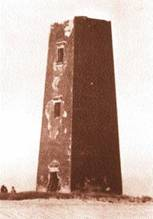
\includegraphics[scale=0.9]{"images/image015.jpg"}
\end{center}

\vskip 4pt

ಆ ಊರಿನವರು ಕೃಷಿಕ ವೃತ್ತಿಯ ಜಾಟ್​ ಸಮುದಾಯದ ಜನ. ಯುದ್ಧ ವೀರರೆಂದೇ ಪ್ರಖ್ಯಾತರಾದವರು ಅವರು. ಇಂತಹ ಸಂದರ್ಭದಲ್ಲಿ, ಬರಿ ಕಾನೂನಿನ ಬಲಾತ್ಕಾರ ಸಲ್ಲ. ಜನರ ಮನವೊಲಿಸಬೇಕು. ಸೂಕ್ತ ಪರಿಹಾರ ಕೊಡಬೇಕು. ತೆರವು ಗೊಳಿಸಬೇಕು. ಅದು ಡಿಸೆಂಬರ್​ ತಿಂಗಳ ಕೊರೆಯುವ ಚಳಿಗಾಲ. ತಕ್ಷಣ ತೆರವುಗೊಳಿದರೂ ಹಳ್ಳಿಯ ಜನ ಡಿಸೆಂಬರ್​ ತಿಂಗಳ ಕೊರೆಯುವ ಚಳಿಯಲ್ಲಿ, ವಸತಿ ಹೀನರಾಗಿ, ಬಯಲಿನಲ್ಲಿ ಬದುಕಬೇಕು. ರಾಮನಗರದ ಹಳ್ಳಿಯಲ್ಲಿ, ಅಡ್ಡ ಬರುತ್ತದೆಂದು ಮೊದಲು ನಿರೀಕ್ಷಿಸಿಯೇ ಇರದ ಮರವೊಂದನ್ನು ಬೀಳಿಸಬೇಕಾದ ಸಂದರ್ಭ ಬಂತು. ಆ ಮರವನ್ನು ಬೀಳಿಸುವಾವಾಗ ಅದು ನಿಯಂತ್ರಣ ತಪ್ಪಿ ನಿರೀಕ್ಷಿಸಿರದ ಇನ್ಯಾವುದೋ ದಿಕ್ಕಿಗೆ ವಾಲಿ ಹೋಗಿ ಗುಡಿಸಿಲುಗಳ ಮೇಲೆ ಬಿದ್ದು ಅದರಿಂದ ಐದು ಗುಡಿಸಲುಗಳು ನಾಶವಾದವು. ಭತೌಣದ \enginline{37} ತಾರಸಿ ಮನೆಗಳು, \enginline{52} ಗುಡಿಸಲುಗಳನ್ನು ನೆಲಸಮ ಮಾಡಲಾಯಿತು. ಜನಕ್ಕೂ ಯಾತನೆ, ಸಂಕಷ್ಟ. ಸರ್ವೇಗೂ ಇದು ದುರ್ಘಟನೆ. ಅಪಾರ ಹಣ ಮತ್ತು ಸಮಯ ಹಾಳು.

\vskip 4pt

ಲ್ಯಾಂಬ್​ಟನ್​ರವರು ಮದರಾಸಿನಿಂದ ಪಶ್ಚಿಮಕ್ಕೆ \enginline{1803}ರಲ್ಲಿ ಟ್ರಾಂಗ್ಯುಲೇಷನ್​ನ್ನು ಮುಂದುವರೆಸುತ್ತಿದ್ದ ಸಮಯ ಅದು. ನಾರ್ನಿಕುಳ ದುರ್ಗದ ಮೇಲೆ ಟ್ರಾಂಗ್ಯುಲೇಷನ್​ ಸ್ಟೇಷನ್​ ಹಾಕಲು ಲ್ಯಾಂಬ್​ಟನ್​ರವರ ಜನ ಅಲ್ಲಿಗೆ ಹೋದರು. ಆದರೆ ಆ ದುರ್ಗವು ಬಂದೂಕು, ಖಡ್ಗ, ಕಠಾರಿಗಳನ್ನು ಹಿಡಿದ ಜನರಿಂದ ರಕ್ಷಿಸಲ್ಪಟ್ಟ ದುರ್ಗವಾಗಿತ್ತು. ಸರ್ವೇ ಮಾಡಲು ಸಹಕರಿಸುವಂತೆ ಇದ್ದ ಲಿಖಿತ ಇಂಗ್ಲಿಷ್​ ಸೂಚನೆಯನ್ನು ಆ ಜನ ಗೇಲಿ ಮಾಡಿದರು. ‘ಇದು ಇಲ್ಲಿಯ ಪಾಳೆಗಾರನ ಹೆಸರಿನಲ್ಲಿರುವ ಪ್ರದೇಶ. ಸರ್ವೇ ಬಾವುಟ ಸೇರಿದಂತೆ ಇತರೆ ಯಾವುದೇ ಬಾವುಟಕ್ಕೆ ಇಲ್ಲಿ ಅವಕಾಶವೇ ಇಲ್ಲ’ ಎಂದರು.

\begin{figure}[!htbp]
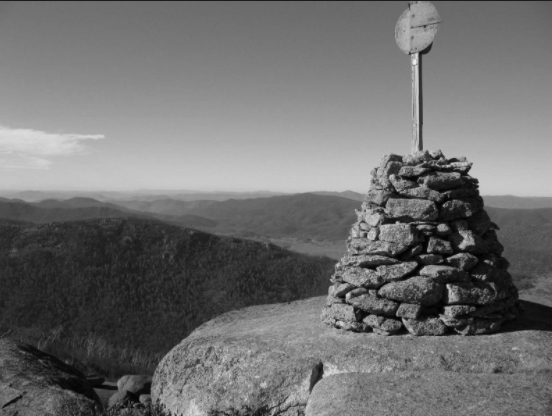
\includegraphics[scale=0.7]{"images/image016.jpg"}
\caption{ಬೆಟ್ಟದ ಮೇಲಿನ ಟ್ರಿಗನಮಿಟ್ರಿಕಲ್​ ಸರ್ವೇ ಸ್ಟೇಷನ್ನಿನ ಸಿಗ್ನಲ್​}\label{art12-fig1}
\end{figure}

\newpage

ಲ್ಯಾಂಬ್​ಟನ್​ರವರ ಜನ ತಕ್ಷಣ ಆ ದುರ್ಗದಿಂದ ಹಿಂತೆಗೆದರು. ಪಕ್ಕದ ಮತ್ತೊಂದು ದುರ್ಗಕ್ಕೆ ಸರ್ವೇ ಸ್ಟೇಷನ್​ ಹುಡುಕಿ ಹೊರಟರು. ಅಲ್ಲೂ ಕೂಡ ಅನುಮತಿ ನಿರಾಕರಿಸಲ್ಪಟ್ಟಿತು. ಈ ಸಲದ ಕಾರಣ ಮಾತ್ರ ಬೇರೆ. ಆ ಕಾರಣ ಏನೆಂದರೆ ಈ ದುರ್ಗದಿಂದ ಪಾಳೇಗಾರನ ಅರಮನೆಯು ನೇರ ವೀಕ್ಷಣೆಗೆ ಒಳಪಡುತ್ತದೆ. ಇದರಿಂದ ಅರಮನೆಯ ಸ್ತ್ರೀಯರು ಪರರ ವೀಕ್ಷಣೆಗೆ ಒಳಗಾಗುತ್ತಾರೆ. ಅವರ ಏಕಾಂತಕ್ಕೆ ತೊಂದರೆ ಆಗುತ್ತದೆ ಎಂದು. ಸ್ಥಳೀಯ ಜನರ ಈ ವಾದದಲ್ಲಿ ಅಷ್ಟೊಂದು ತಪ್ಪು ಇಲ್ಲವೆನ್ನಬಹುದು. ಏಕೆಂದರೆ, ಈ ಸರ್ವೇ ಉಪಕರಣದ ಟೆಲಿಸ್ಕೋಪು, ದೂರದಲ್ಲಿನಅ ವಸ್ತುಗಳನ್ನು ದೊಡ್ಡದು ಮಾಡಿ ಸಮೀಪದಲ್ಲೇ ಇರುವಂತೆ ತೋರಿಸುತ್ತಿತ್ತು. ಅಷ್ಟೇ ಅಲ್ಲ, ಸ್ತ್ರೀಯರು ಮಕ್ಕಳು ಸೇರಿದಂತೆ ನೋಡಿದ ಎಲ್ಲರನ್ನೂ, ಎಲ್ಲವನ್ನೂ ತಲೆಕೆಳಗು ಮಾಡಿ ತೋರಿಸುತ್ತಿತ್ತು.

ಇಂತಹ ಸರ್ವೇಯು ಕೆಲವೊಮ್ಮೆ ಹಳ್ಳಿಗಳಲ್ಲಿ ಆತಂಕಕ್ಕೂ ಸಹ ಕಾರಣವಾಗುತ್ತಿತ್ತು. ಸರ್ವೇ ತಂಡಕ್ಕೆ ಸಾಮಾನ್ಯವಾಗಿ ಬೆಟ್ಟ ಅಥವಾ ದುರ್ಗದ ನೆತ್ತಿಯೇ ಬೇಕು. ಬೆಟ್ಟದ ನೆತ್ತಿಯಲ್ಲಿ ದೀಪಗಳನ್ನು ಹಚ್ಚಿಕೊಂಡು ವೀಕ್ಷಣಾ ಕಾರ್ಯ ಮಾಡಲಾಗುತ್ತಿತ್ತು. ದೀಪವನ್ನು ಬಳಸಿ, ರಾತ್ರಿ ಸಮಯದಲ್ಲೂ ವೀಕ್ಷಣೆ ಮಾಡುವ ವಿಧಾನವನ್ನು ಎವರೆಸ್ಟ್​ರವರು ಹೊಸದಾಗಿ ಶೋಧಿಸಿದ್ದರು. ಸಾಮಾನ್ಯವಾಗಿ ಈ ಬೆಟ್ಟದ ಟ್ರಿಗನಮಿಟ್ರಿಕಲ್​ ಸ್ಟೇಷನ್​ ತಾಣಗಳು ಸ್ಥಳೀಯ ದೇವ ದೇವತೆಗಳ ಸ್ಥಾನಗಳೂ ಹೌದು. ಎವರೆಸ್ಟ್​ರವರ ರಾತ್ರಿ ಕಾರ್ಯವು ಹಳ್ಳಿ ಜನರಲ್ಲಿ ಅನುಮಾನ ಮೂಡಿಸುತ್ತಿದ್ದವು. ಗುಡಿಯ ಪೂಜಾರಪ್ಪನ ಮಾತು ಸಹ ರೈತಾಪಿ ಜನರಲ್ಲಿ ಶಂಕೆಯನ್ನು ಹೆಚ್ಚು ಮಾಡುತಿದ್ದವು. ‘ನಡುರಾತ್ರಿಯಲ್ಲಿ ಬೆಟ್ಟದ ನೆತ್ತಿಯಲ್ಲಿ ಬೆಂಕಿ ಹಿಡಿದು ಕೂರುವುದು, ಇದು ನಮ್ಮ ಊರಿನ ದೇವತೆಯಲ್ಲಿ, ಹೊರ ಊರಿನ ಮಾಟಗಾರರು ನಡೆಸುತ್ತಿರುವ ಯಾವುದೊ ಮಾಟ ಮಂತ್ರ. ಇದರಿಂದ ನಮ್ಮ ದೇವತೆಯು ಮುನಿಯಬಹುದು. ಊರಿಗೆ ಕೇಡಾಗಬಹುದು.’ ಇದು ಹಳ್ಳಿ ಜನರ ಮುಂದೆ ಪೂಜಾರಪ್ಪನ ಅಳಲು. ಹಳ್ಳಿಯ ಮುಗ್ಧ ಜನಕ್ಕೆ ಇಷ್ಟೇ ಸಾಕು. ಸರ್ವೇ ತಂಡ ತನ್ನ ವೀಕ್ಷಣೆ ಕಾರ್ಯ ಮುಗಿದ ನಂತರ, ಅಲ್ಲಿ ಕೋನ ಓದಿದ ಸ್ಟೇಷನ್​ಗಳಲ್ಲಿ ಗುರುತು ಮಾಡುವುದು ಕ್ರಮ. ಈ ಕ್ರಮ ಏನೆಂದರೆ, ಹರಿತ ಉಳಿಯಿಂದ ಬಂಡೆಯ ಮೇಲೆ ಸರ್ಕಲ್​ ಮತ್ತು ಡಾಟ್​ ಗುರುತನ್ನು ಕೆತ್ತಿ, ಅದರ ಮೇಲೆ ಸರ್ವೇ ಸಿಗ್ನಲ್​ ಇಟ್ಟು, ಸುತ್ತ ಕಾಡುಗಲ್ಲುಗಳಿಂದಲೇ ಸಣ್ಣದೊಂದು ಪ್ಲಾಟ್​ಫಾರಮನ್ನು ಕಟ್ಟಲಾಗುತ್ತದೆ. ಆ ಪ್ಲಾಟ್​ಫಾರಮ್ಮಿನ ನಡುವೆ ಸಿಗ್ನಲ್ಲು ನೇರವಾಗಿ ಕೆಳಗಿನ ಮಾರ್ಕ್ ಮೇಲೆಯೇ ಬರುವಂತೆ ನೆಟ್ಟಗೆ ನಿಲ್ಲಿಸಲಾಗುತ್ತದೆ. ನಂತರ ಸರ್ವೇ ತಂಡವು ಅತ್ತ ಮುಂದಿನ ಸ್ಟೇಷನ್ನಿನ ಕಡೆಗೆಅ ಮುನ್ನಡೆಯುತ್ತದೆ. ಇತ್ತ ಹಳ್ಳಿ ಜನ ಬಂದು ಆ ಸರ್ವೇ ಸ್ಟೇಷನನ್ನು ನೋಡುತ್ತಾರೆ. ಏನೋ ಹೊಸದಾಗಿ ಕಟ್ಟಿದ ಕಲ್ಲಿನ ರಾಶಿ ಮತ್ತು ನಿಗೂಢವಾಗಿ ನೆಟ್ಟ ಬಾವುಟ. ಅದು ಏನೆಂದು ಹಳ್ಳಿಯ ಜನರಿಗೆ ಒಂದೂ ಅರ್ಥವಾಗುವುದಿಲ್ಲ. ಆ ಫ್ಲಾಗನ್ನು ಕಿತ್ತು ಬಿಸಾಕಿ ಅಸ್ತವ್ಯಸ್ತಗೊಳಿಸಿದಾಗಲೇ ಅವರಿಗೆ ಸಮಾಧಾನ. ಅತ್ತ ಹೊರಟ ಸರ್ವೇ ತಂಡ ಹಿಂದಿನ ಸ್ಟೇಷನ್​ ಮೇಲೆ ಪುನಃ ವೀಕ್ಷಣೆ ಮಾಡಲು ಬಾವುಟವನ್ನು ನೋಡಿದರೆ, ಸರ್ವೇ ಗುರುತು ನಾಶವಾಗಿರುತ್ತದೆ. ಅದನ್ನು ಪುನರ್​ ನಿಗಧಿ ಮಾಡುವುದು, ಮತ್ತೂ ಆಳಕ್ಕೆ ಕಲ್ಲಿನಲ್ಲಿ ಕೊರೆಯುವುದು, ಇನ್ನೊಮ್ಮೆ ಫ್ಲಾಗನ್ನು ನೆಡುವುದು, ಈ ಪುನಾರಾವರ್ತನೆಯ ಕೆಲಸವನ್ನು ಮಾಡಬೇಕಾಗುತಿತ್ತು. ಇದರಿಂದ, ಸಾಮಾನ್ಯವಾಗಿ ನಿಧಾನದ ಸರ್ವೇ ಕಾರ್ಯವು ಮತ್ತಷ್ಟು ವಿಳಂಬಕ್ಕೆ, ಸಂಕಷ್ಟಕ್ಕೆ ಕಾರಣವಾಗುತ್ತಿತ್ತು.

ಗ್ರಾಮೀಣ ಭಾರತೀಯರು ಸರಳ ಮನಸಿನವರು. ಸರ್ವೇ ಕಾರ್ಯ ನಡೆಯುತಿದ್ದ ಊರಿನ ಸ್ಥಳೀಯ ಜನರು ಸರ್ವೇ ಕಾರ್ಯವನ್ನು ಸದಾ ಅನುಮಾನದಿಂದಲೇ ನೋಡಿದರು ಅಂತಲೂ ಅಲ್ಲ. ಇಂತಹ ಘಟನೆಗೆ ವ್ಯತಿರಿಕ್ತವಾಗಿ, ಸರ್ವೇ ಕಾರ್ಯಕ್ಕೆ ಸಹಕರಿಸಿದ ಅನೇಕ ಸಂದರ್ಭಗಳೂ ಸಹ ಸಾಕಷ್ಟು ಇವೆ. ಜೊತೆಗೆ, ಎವರೆಸ್ಟ್​ರವರು ಚಂಬಲ್​ ಕಣಿವೆ ಪ್ರದೇಶದಲ್ಲಿ ಟ್ರಾಂಗ್ಯುಲೇಷನ್​ ಕಾರ್ಯ ನಡೆಸುತ್ತಿದ್ದಾಗ, ಅವರ ಗ್ರೇಟ್​ ಥಿಯಡೋಲೈಟನ್ನು ಅಲ್ಲಿನ ಕಣಿವೆಯ ಮುಗ್ಧ ಜನ ಬಂದು ನೋಡಿ, ಸಂಭ್ರಮಿಸಿದ್ದಿದೆ. ಭಯದಲ್ಲಿ ಗ್ರೇಟ್​ ಥಿಯಡೋಲೈಟಿಗೆ ಗೌರವವನ್ನು ಅರ್ಪಿಸಿದ ಉದಾಹರಣೆಯೂ ಇದೆ.

